\chapter{Introduction}
\label{ch:introduction}
\setcounter{footnote}{0}
The Greek philosopher Heraclitus once said that one constant since the beginning of time is change. However, the fear of change is also a constant.  His central claim is summed up in the phrase Panta Rhei ("life is flux"), recognising life's essential, underlying essence as change\footnote{\url{https://plato.stanford.edu/entries/process-philosophy/}}. Nothing in life is permanent, nor can it be, because the very nature of existence is change. Since times \gls{immemorial}, humans have liked routine, making us feel in control of our lives. When that fear of change becomes irrational, our ability to control it becomes a phobia, particularly Metathesiophobia. A Metathesiophobe feels they have no control over their lives due to constant change. Metathesiophobes tend to live in the past and are unwilling to progress, often leading to depression, seriously impacting their professional and personal lives \parencite{PsychTimes}. If a society or country rejects the change, there is no growth and no progress. According to \textcite{Mark2010}, the inability to change, progress, or grow can result in stagnation. Stagnation rejects realising ones full potential.

A world that is continuously in flux is a volatile, uncertain, complex and ambiguous world \parencites{Bennett2014}{Sinha2020}. According to \textcite{Bennett2014} the world of \acrfull{vuca} requires a new approach. \Gls{disintermediation}, globalisation, market upheaval, disruption, and technological advance all combine to produce an effect that is difficult to mitigate,  impossible to predict, and \gls{arduous} to detect \parencite[p.~885]{OReilly2019}. \textcite{Taleb2008} his definition of a \gls{blackswan}, \cref{sec:introantifragility}, is similar. To deal with the \acrshort{vuca} world, companies invested a great deal of time and money in becoming less \gls{fragile} by being more \gls{robust} and \gls{resilient}. However, \textcite{Taleb2012} claims that by being more \gls{robust}, or \gls{resilient}, the company can only withstand the change but does not gain from it.

\textcite{Taleb2012} defines the opposite state of \gls{fragile}, \gls{antifragile} as an answer to what \textcite{Taleb2008} calls \glspl{blackswan}. According to \textcite{Taleb2012} \gls{resilient}, \gls{robust} (and company) are states that neither breaks nor improves. \textcite{Taleb2012} claims that \gls{antifragile} is the state that gains and improves. \Gls{antifragile} is the true opposite of \gls{fragile}.

In this thesis, I define the success factors that have a positive influence on \acrfull{ea} to contribute to achieving \gls{antifragility} in the public sector.
\section{Author}
\label{sec:author}
I am working as a \gls{chiefarchitect} for an \acrfull{isv} delivering products and services to the local governmental agencies in The Netherlands, such as municipalities, the local tax offices, and the social services. I am responsible for the architecture function of this company. With architecture, we use an outside-in approach. We monitor our external environment, the public sector, and translate this into changes for our organisation, services and products. We do this to stay relevant in the market we serve, the public sector. I find the aspect of public responsibility important in my day to day work. Civilians and companies eventually pay every euro spent on a product or service based on taxes. If we can deliver our products and services more efficiently and more effectively, the better the public money is spent. Delivering products and services in the public sector is influenced by the changes the public sector is going through. These changes can be planned changes but also changes needed based on \glspl{stressor}, e.g. \cref{fig:publicstressors}. \Gls{antifragile} can help us to get better and adapt to those changes more quickly, and by doing so, make changes more efficiently and more effective with a result of spending less public money.
\section{Structure}
\label{sec:structure}
In \cref{ch:introduction}, the context of the research is set, the core concepts of \acrshort{ea} and \glspl{antifragile} are introduced together with the the public sector. The chapter states the problem statement, the research questions, and the substantiation of the relevance of the research. In \cref{ch:theoreticalbackground}, the background on the concepts is given. The lens of the public sector is defined. \cref{ch:methodology} explains the used research methodology and the approach for the research. \cref{ch:attributes} describes the found attributes from the literature that can be success factors. \cref{ch:attributes} ends with an overview of found attributes of \acrshort{ea} and \gls{antifragile} that could contribute to the public sector to become \gls{antifragile}. These attributes are the point of departure for further investigation. \cref{ch:interviews} gives a summary of the conducted interviews together with the findings from the interviews. The interviews are validated. The output of the interviews extends the list of attributes with new findings. \cref{ch:expertgroup} is about the outcome of the expert group. This chapter includes possible new findings and the validation of the output of the expert group. The \cref{ch:alysis} brings the outcomes from the literature study, interviews and expert group together for analysis. The possible success factors are defined, weighted, and screened to determine a set of success factors by triangulation. Finally, the conclusion, discussion and recommendations are in \cref{ch:conclusionanddiscussions}. This thesis ends with \cref{ch:retrospective} for a retrospective of the researcher, the research, and its process. To support the reader of this thesis with mutual understanding on definitions this thesis contains a glossary of terms.
\section{Introduction of the public sector}
\label{sec:intropublicsector}
According to \textcite{PrivacySense2016} the public sector is comprised of organisations that are owned and operated by the government and exist to provide services for its citizens. Similar to the non-profit sector, organisations in the public sector do not seek to generate a profit. \textcite{PrivacySense2016} divides the public sector into three levels.
\begin{itemize}
	\item{\textbf{The national government,} such as the military, the tax authority, and homeland affairs.}
	\item{\textbf{The regional government,} such as the provinces, the police, and water management.}
	\item{\textbf{The local government,} such as the municipalities, the social services, and the local tax offices.}
\end{itemize}
For this research the lens is set to the public sector consisting out of the national governments, the local governments and the suppliers delivering services to these governmental agencies. The national governments because they are responsible for policy making while the local governments are responsible for executing most of those policies.
\section{Introduction of the concept Enterprise Architecture}
\label{sec:introea}
\textcite[p.~104]{Lapalme2016} says that \acrfull{ea} should be understood as being constituted of the essential elements of a socio-technical organisation, their relationships to each other and their changing environment, as well as the principles of the organisation’s design and evolution. Enterprise architecture management is the continuous practice of describing and updating the \acrshort{ea} to understand the complexity and manage change \parencite{Lapalme2016}. 
\section{Introduction of the concept of antifragility}
\label{sec:introantifragility}
\textcite{Taleb2008} describes a \gls{blackswan} as an event that is so rare that even the possibility that it might occur is unknown, has a catastrophic impact when it does occur, and is explained in hindside as if it were predictable \parencite[p.~4]{Taleb2012}.
\begin{enumerate}
	\item{is so rare that even the possibility that it might occur is unknown,}
	\item{has a catastrophic impact when it does occur,}
	\item{is explained in hindsight as if it were predictable.}
\end{enumerate}
For extremely rare events, \textcite{Taleb2008} argues that the standard tools of probability and prediction, such as the normal distribution, do not apply since they depend on a large population and past sample sizes that are never available for rare events by definition. Using statistics based on extrapolating observations of past events does not help predict black swans and might even make us more vulnerable to them. In his book \Gls{antifragile}, \textcite{Taleb2012} states that the way to survive a black swan event is to be \gls{antifragile}.

Most people answer that the opposite of \gls{fragile} is \gls{robust}, \gls{resilient}, solid, or something of the sort. However, the \gls{resilient}, \gls{robust} (and company) are items that neither break nor improve. As seen in \cref{fig:antifragilesimple}, the exact opposite of something that is \gls{fragile} is not only unbreakable, but it would benefit from shocks and a wide array of trauma \parencite{Taleb2012}. It does not lose, but it gains. \textcite{Taleb2012} defines something that gains from shocks and a wide array of trauma as \gls{antifragile}. 
\begin{figure}[H]
	\centering
	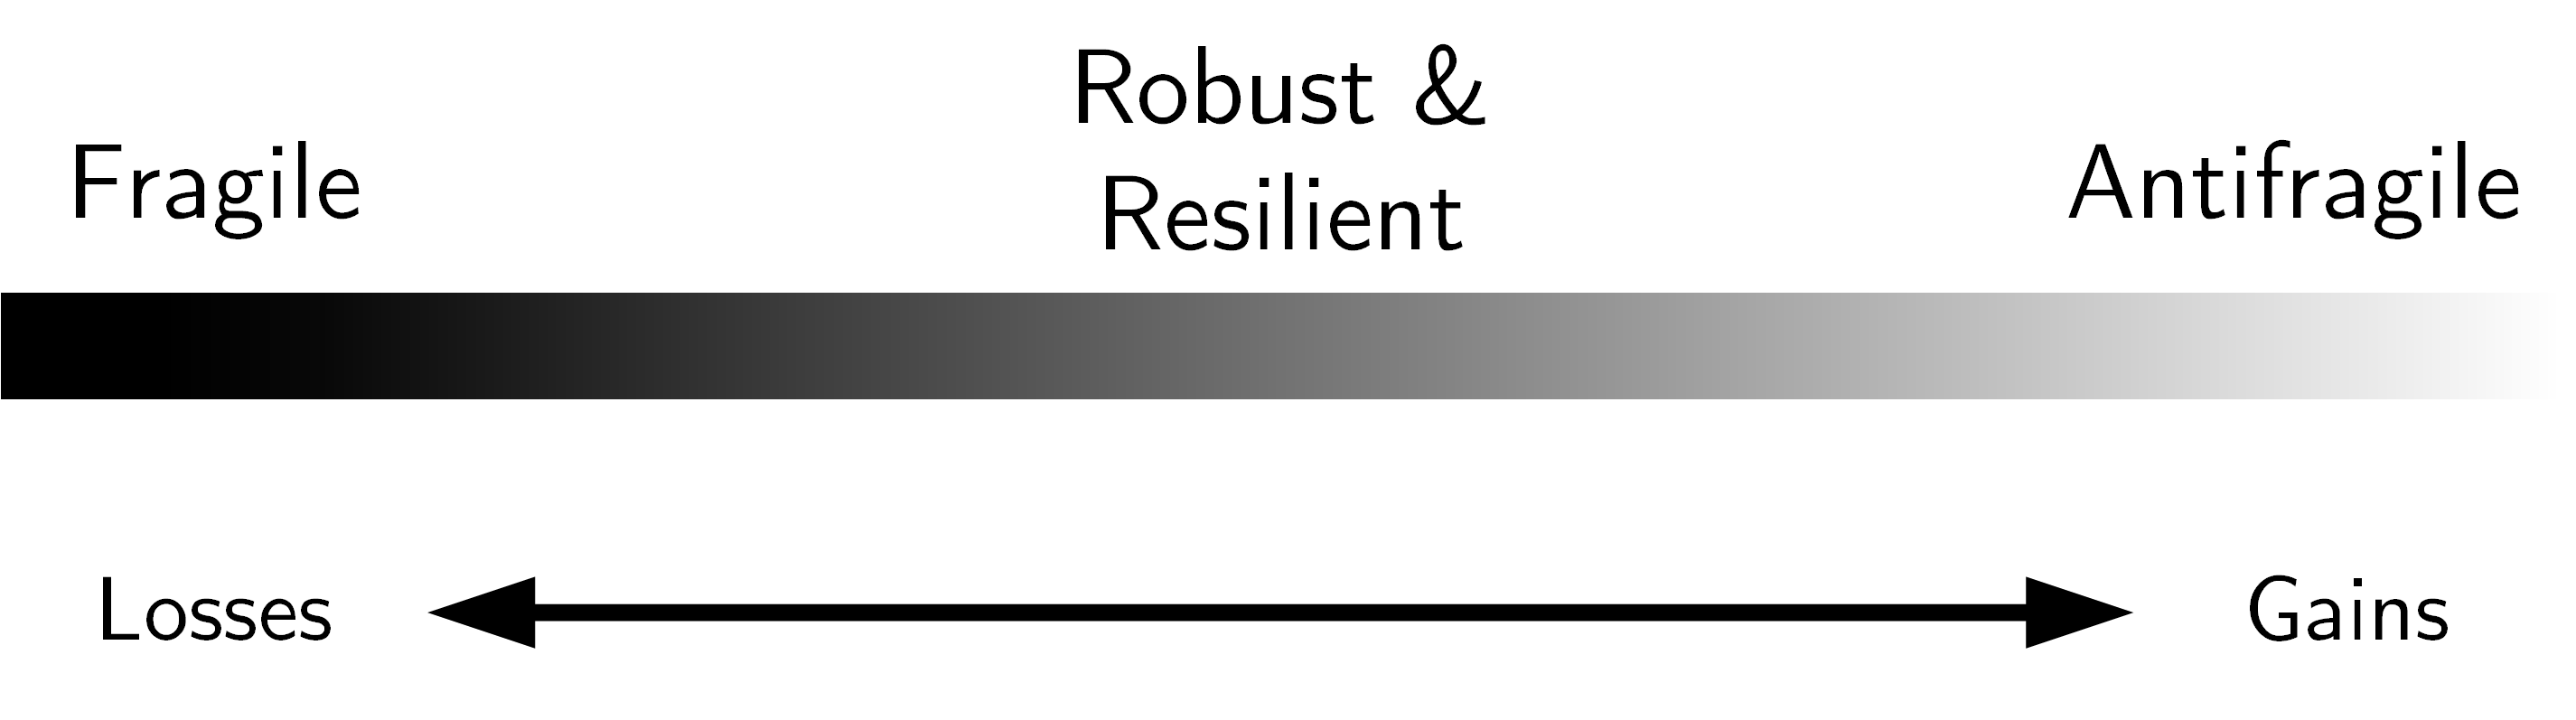
\includegraphics[width=0.6\linewidth]{images/antifragilesimple}
	\caption[The opposite of fragile]{The opposite of fragile}
	\label{fig:antifragilesimple}
\end{figure}
\section{Problem statement}
\label{sec:problemstatement}
The concept of \gls{antifragility} implies that organisations could benefit and strengthen from crises, volatility, errors and uncertainty and could also lead to opportunities for innovation \parencite{Kastner2017}. \acrshort{ea} is a discipline that helps organisations to reach their goals. As described in \cref{sec:introea}, with \acrshort{ea}, an organisation can understand the complexity and manage change. One would expect that an organisation can use \acrshort{ea} to get more towards the state of \gls{antifragility}. The current \acrfull{bok} of \acrshort{ea} and \gls{complexityscience} does contain some research on \gls{antifragility} on application and information architectures but not on \acrshort{ea}. The \acrshort{bok} is not containing knowledge on how to achieve \gls{antifragility} with the use of \acrshort{ea}.
\section{Research subject}
\label{sec:researchsubject}
As described in \cref{sec:introea},  \acrshort{ea} is an approach for controlling the complexity and constant changes in the business environment of an organisation, enabling alignment between the business vision, business requirements and information systems. So \acrshort{ea} facilitates an organisation in assessing the impact of change and making recommendations for target states that support business objectives. \acrshort{ea} can help organisations in changing towards the state of \gls{antifragility}.

However, what are the success factors of \acrshort{ea} and \gls{antifragile} that have a positive influence on \acrshort{ea} to contribute in achieving \gls{antifragility} in the \gls{ps}? 
\begin{figure}[H]
	\centering
	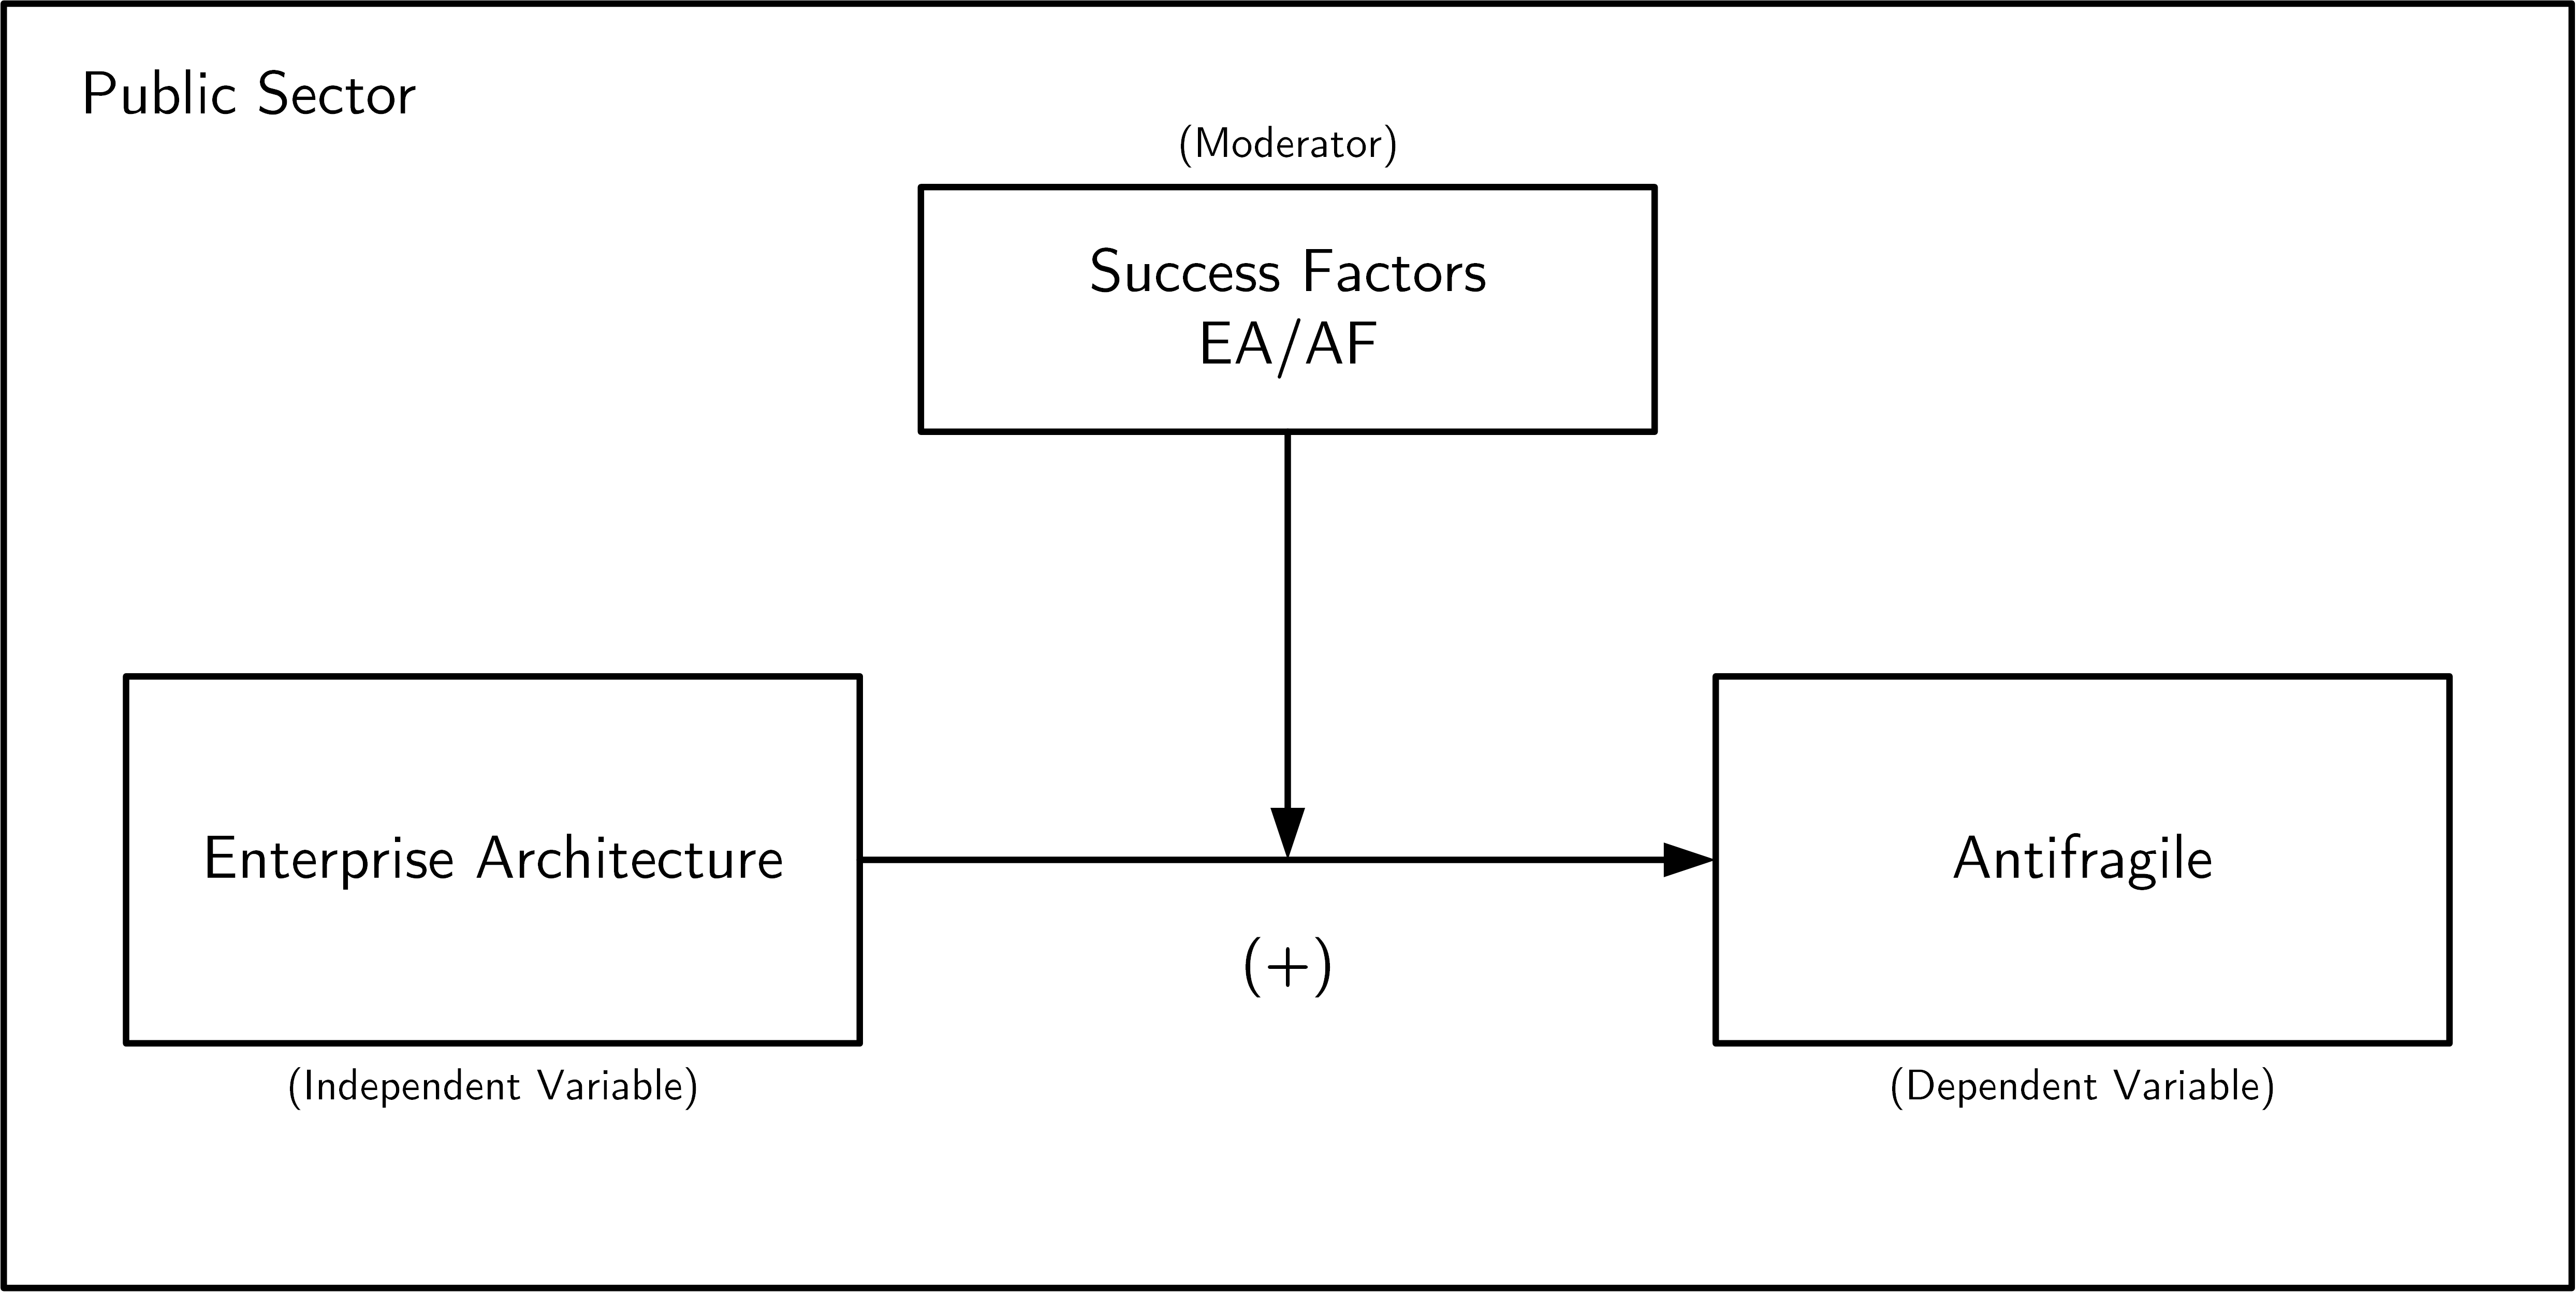
\includegraphics[width=0.7\linewidth]{images/conceptualmodel}
	\caption[Conceptual Research Model]{Conceptual Research Model}
	\label{fig:conceptualmodel}
\end{figure}
\section{Research question}
\label{sec:introresearchquestion}
 The conceptual research model (\cref{fig:conceptualmodel}) describes the hypothesises that, in the context of the public sector, there are success factors of \acrshort{ea} and \gls{antifragile} that have a positive influence on the contribution of \acrlong{ea} in achieving \gls{antifragility}. Following the conceptual research model, the following research question is determined:\bigskip

\noindent \emph{''What are the success factors that positively influence the contribution of \acrlong{ea} in achieving \gls{antifragility} in the \gls{ps}?''}\bigskip

\noindent The following sub-questions support answering the research question:

\begin{enumerate}
	\item{What is the literature saying about the \gls{ps}?}
	\item{What is the literature saying about \gls{antifragile}?}
	\item{What are the possible success factors of \gls{antifragile}?}
	\item{What is the literature saying about \acrlong{ea}?}
	\item{What are possible success factors of \acrlong{ea}?}
	\item{Which success factors can positively influence the contribution of \acrlong{ea} in achieving \gls{antifragility} in the \gls{ps}?}
\end{enumerate}
\section{Research relevance}
\label{sec:researchrelevance}
\acrshort{ea} has contributed to organisations in being more \gls{robust}, and \gls{resilient}. Using \acrshort{ea} in pursuing \gls{antifragility} will add value to companies by accelerating and growing when there is a \gls{stressor} or a \gls{blackswan}. For some examples of \glspl{stressor} which are relevant to the \gls{ps} see \cref{fig:publicstressors}. The \gls{antifragile} theory is young. \citeauthor{Taleb2012} published the theory in his book ''\Gls{antifragile}: Things that gain from disorder.'' in \citeyear{Taleb2012}. Studies conducted on \acrshort{ea} with the concept of \gls{antifragile} are almost non-existence. The conducted studies are primarily about making IT Systems \gls{antifragile}. \textcites{Botjes2020}{Kastner2017} are exceptions and have researched how to apply \gls{antifragile} in an organisational context. Nevertheless, both concluded that there is more research needed. The former used the lens of Enterprise Engineering, which is closely related to \acrshort{ea}, together with complex adaptive system resilience, while the latter used mostly resilience as its lens. There is still no answer to how \acrshort{ea} can contribute to achieving \gls{antifragility}. Giving more insights on this subject will contribute to the \acrshort{bok} of \acrshort{ea} and \gls{complexityscience} and help others get closer to \gls{antifragility} by using \acrshort{ea}.
{\let\thefootnote\relax\footnote{{\url{https://www.istockphoto.com/en/vector/506120634-84046799}}}}
\begin{figure}[H]
	\centering
	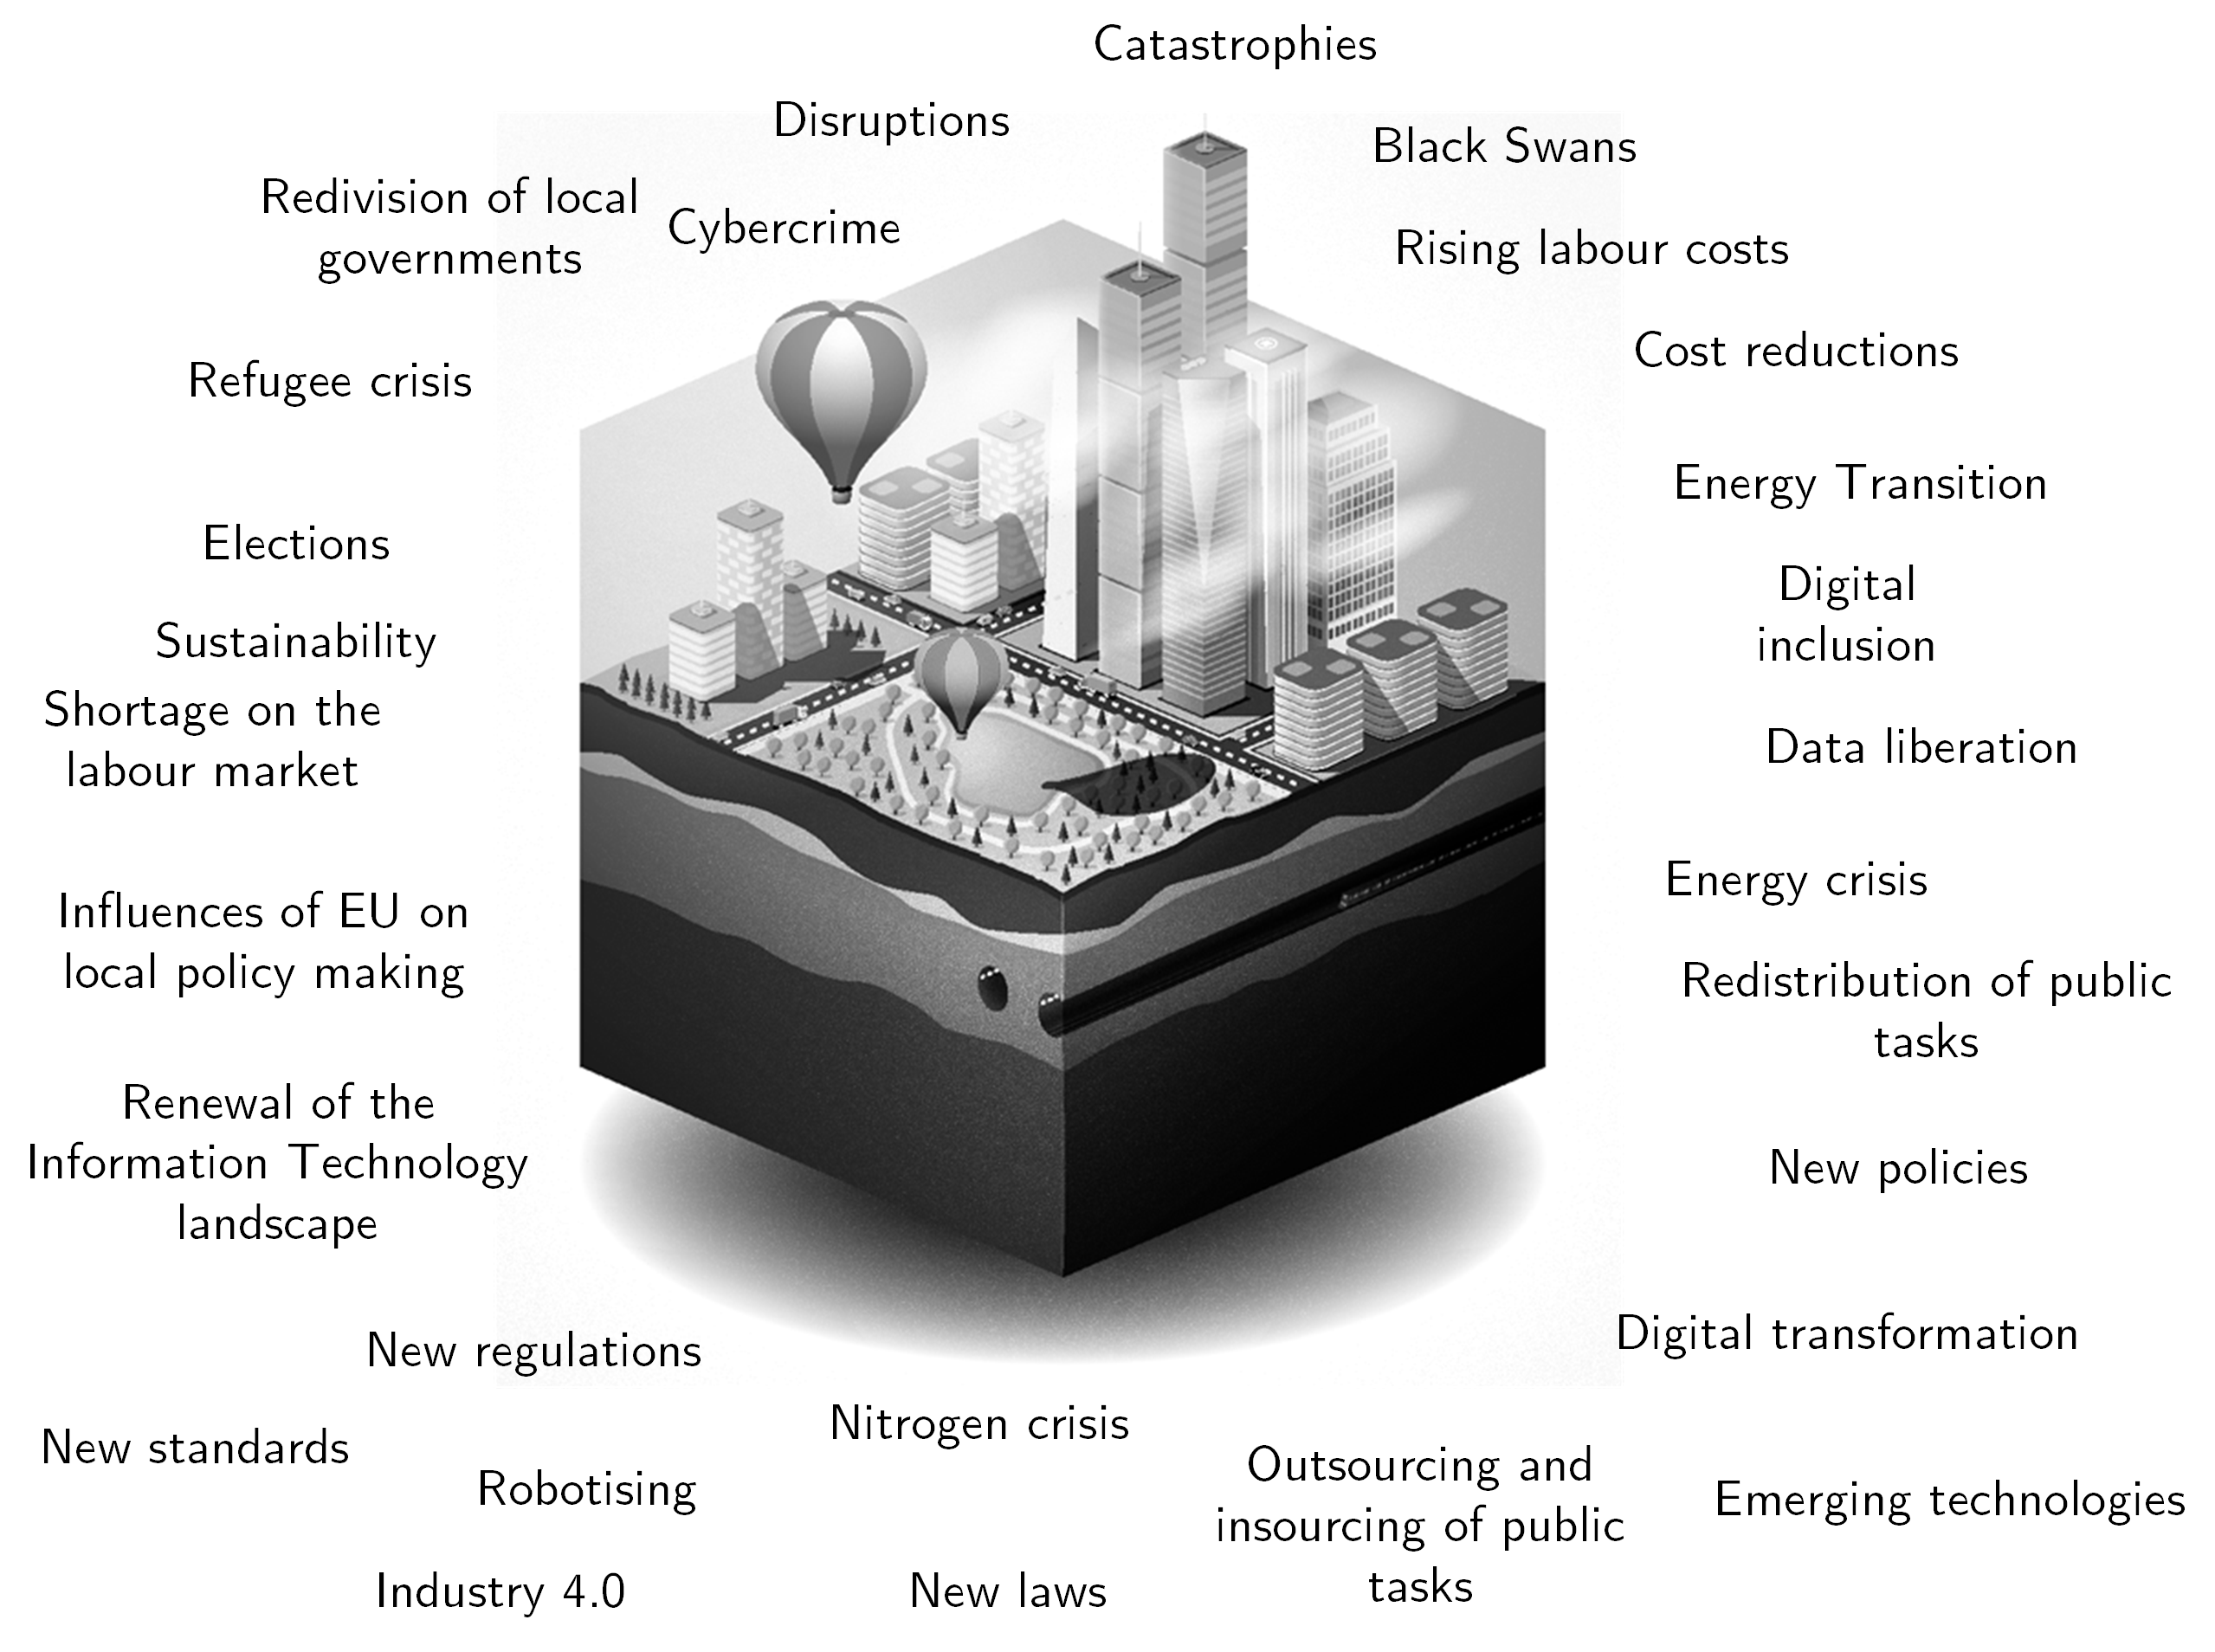
\includegraphics[width=0.8\linewidth]{images/publicstressors}
	\caption[Examples of stressors on the public sector]{Examples of stressors on the public sector}
	\label{fig:publicstressors}
\end{figure}
Because of the \gls{digitaltransformation}, the pace of change is increasing rapidly. In a study by \textcite{Eggers2015}, 96\% of respondents said digital technologies are significantly disrupting the \gls{ps}. According to \textcite{Nurmi2021}, organisations in the public and private sectors alike face the need to manage themselves in an ever more interconnected and fast-paced world. \textcite{Guggenberger2020} states that a paradigmatic change from a mechanistic toward a systemic worldview is ongoing, emphasizing the interconnectedness of participating organizations. The \gls{digitaltransformation} is not the only \gls{stressor} on the \gls{ps}. There are a lot of internal and external \glspl{stressor}. By being more \gls{robust} or \gls{resilient}, you can only withstand the change or the \gls{stressor}, but you do not gain from it. Governmental organisations and agencies in the Dutch \gls{ps} are searching for methods of dealing with this increased pace and the stressors. There are a lot of indications of this in the discussions and sessions held at ''the iBestuur congress of 2021''\footnote{\url{https://magazine.ibestuur.nl/ibestuur_congres_2021_terugblik/cover}}. The relevance of this research is not only about adding to the \acrshort{bok} of \acrshort{ea} and \gls{complexityscience} but also, in the context of public responsibility, to share the outcome with the \gls{ps} for further study and use.